\documentclass[conference]{IEEEtran}
\IEEEoverridecommandlockouts
% The preceding line is only needed to identify funding in the first footnote. If that is unneeded, please comment it out.
\usepackage{cite}
\usepackage{longtable}
\usepackage{amsmath,amssymb,amsfonts}
\usepackage{algorithmic}
\usepackage{graphicx}
\usepackage{textcomp}
\usepackage{longtable}


\def\BibTeX{{\rm B\kern-.05em{\sc i\kern-.025em b}\kern-.08em
    T\kern-.1667em\lower.7ex\hbox{E}\kern-.125emX}}
\begin{document}
 \title{Restaurant Management System}
\author{\IEEEauthorblockN{Anmol R.Sajnani,}
	\IEEEauthorblockA{B.Tech Integrated\\Computer Engineering,\\MPSTME, NMIMS\\anmolsajnani04@gmail.com}
	\and
	\IEEEauthorblockN{Hitesh M.Jeswani,}
	\IEEEauthorblockA{B.Tech Integrated\\Computer Engineering,\\MPSTME, NMIMS\\hiteshjeswani112@gmail.com}
	\and
	\IEEEauthorblockN{Manan R.Mehta,}
	\IEEEauthorblockA{B.Tech Integrated\\Computer Engineering,\\MPSTME, NMIMS\\mehtamanan0@gmail.com}
	}
\maketitle
 
 
\begin{abstract}
There is a saying “the best interface is no interface,” many people are considering voice interface as an excellent approach to reduce friction of Chatbot. Natural Language Processing system takes human understandable language as input and converts it into machine coherent code. This code is then processed and translated back to natural language. A major problem faced by the customers in a restaurant is waiting for the staff to take order, this is because during rush hours the availability of staff decreases. This mishap can be removed by implementing a restaurant management system which is presented in this paper. Techniques like NLP, Rule-based system, deep-learning algorithms, Sentiment Analysis are used in the proposed framework.\\
\end{abstract}
\begin{IEEEkeywords}
	Sentiment Analysis(SA), Machine Learning(ML), Deep Learning(DL), Automatic Speech Recognition(ASR), Text to Speech(TTS)
\end{IEEEkeywords}
\section{Introduction}
Nowadays hustling restaurants take a lot of time to process the given order and also the time it takes to collect the order from all the tables during rush hours increases with the number of tables occupied. We came with a solution to this problem with the help of a restaurant management system deployed using NLP, ML, DL, and Rule Based System. 
Focus of this project is to build a device which can help restaurants in optimizing their profits by providing following functionalities:
\begin{itemize}
	\item A computing device interacting with the customers, taking order from them, asking their preferences. This reduces human labour and increases the enjoyment of bon vivante in the restaurant.
	\item Applying Sentiment Analysis to the customer’s reviews and feedback can provide restaurants knowledge about areas of improvement and different price ranges.
\end{itemize}
\begin{figure}[!ht]
	\centering
	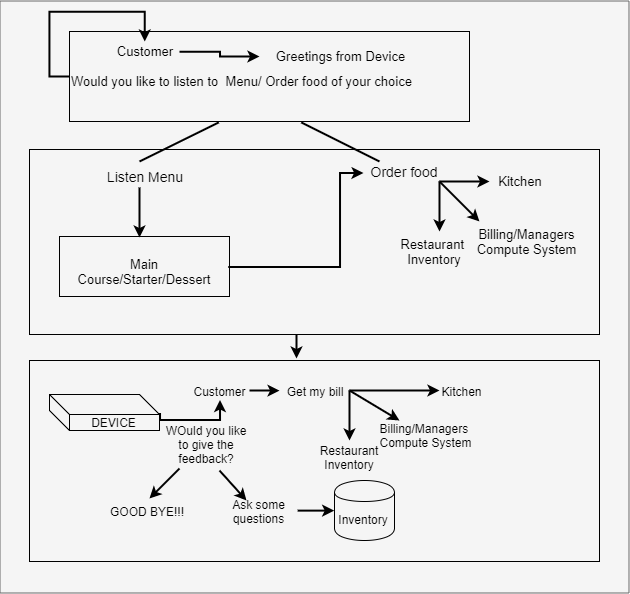
\includegraphics[width=0.5\textwidth]{overview.png}
	\caption{ Flowchart for the proposed System}
\end{figure}
NLP takes order as voice commands and converts them to text, this data is stored in the DB and sent to management server where the data is processed. Order is sent to the kitchen and when it is ready, order is sent to the customer directly. Once the customer is satisfied with the food and asks for bill, bill is presented to the customer along with an option to provide feedback about the food or not. If the customer opts for providing the feedback, Sentiment Analysis algorithm is orchestrated in the background to scrutinize the feedback provided by the user. Now when sufficient feedbacks are gathered from various customers, restaurant authorities can come to know what kind of food people like, what is currently in the demand. These NLP systems are installed on all the tables and now the customers can interact with the system hands-free. \\
The implementation of such a system will lead to major advantages: 
\begin{itemize}
	\item During rush hours multiple customer requests will be handled efficiently without the customer having to wait to place the order. 
	\item This system eliminates the overhead of waiter taking orders from the customer and the human-errors encountered in the process. 
\end{itemize}


\section{Literature Survey}

\subsection{\textbf{Speech Recognition}}
In Speech Recognition technology speech given as an input is converted to text, Automatic Speech Recognition is used for that purpose. Automatic Speech Recognition (ASR) can be defined as the independent, computer-driven transcription of spoken language into readable text in real time. ASR is technology that allows a computer to identify the words that a person speaks into a microphone or telephone and convert it to written text. Although ASR technology is not yet at the point where machines understand all speech, in any acoustic environment, or by any person. It is used on a day-to-day basis in a number of Natural Language Processing applications and services. 
The ultimate goal of ASR research is to allow a computer to recognize in real-time, with 100\% accuracy, all words that are intelligibly spoken by any person, independent of vocabulary size, noise, speaker characteristics or accent. Today, if the system is trained to learn an individual speaker‘s voice, then much larger vocabularies are possible and accuracy can be greater than 90\%. Most commercial companies claim that recognition software can achieve between 98\% to 99\% accuracy if operated under optimal conditions. Optimal conditions usually assume that users have speech characteristics which match the training data, can achieve proper speaker adaptation, and work in a clean noise environment \cite{b1}. 
Figure 2 shows the block diagram of a typical ASR system. It is composed of two major components: the front end and the decoder. The front end block extracts spectrum representation of the speech waveform. The most widely used features are Mel Frequency Cepstral Coefficients (MFCC)\cite{b2}. The decoder block searches the best match of word sequences for the input acoustic features based on acoustic model, lexicon, and language model. 
\begin{figure}[!ht]
	\centering
	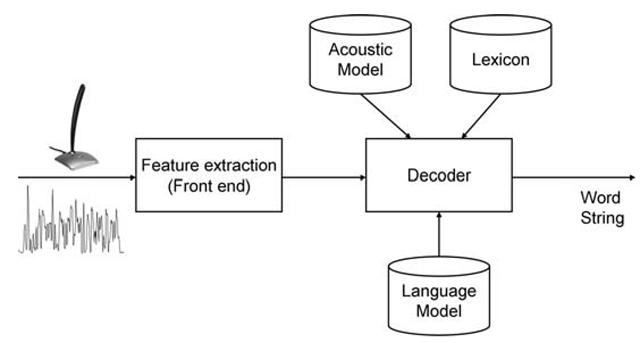
\includegraphics[width=0.222\textwidth]{ASR.png}
	\caption{Automatic Speech Recognition System\cite{b3}}
\end{figure}\\
\subsection{\textbf{AI response module}}
Our current Rule Based System involves the following approaches:
\begin{itemize}
	\item rule based system
	\item seq2seq outlier request handling model
\end{itemize}

\bigskip

\textbf{\textit{Rule based system}}

\bigskip

Our rule based system will first get the input text from the "speech to text module" and this text will be run on an entity detection module in order to generate the given meaning of the sentence. The intent will signify the meaning of the sentence in order to maintain the conversation flow. Once the intent is determined the rule based system will generate an output response in relation to the intent. While the text is being processed, the entities will be recorded such as "1 burger" in order to calculate the bill.

\bigskip

\textbf{\textit{seq2seq outlier request handling model}}

The seq2seq model helps in handling the outlier queries. The model will receive the queries once the rule based system detects that the intent for the given input text is an outlier intent. The seq2seq model will generate a suitable response instead of a default response.

\bigskip

\subsubsection{Training data}
The model was trained on the twitter data corpus in order to have a generalized dataset. This dataset captures normal conversations that might not be specific to the food ordering system.

\bigskip

\subsubsection{Model generation}
The code is written in python and the Tensorflow library is used.
The data is provided in an encoding and a decoding format. Where the data will be tagged according to weather it is for an encoding format or a decoding format.

\begin{figure}[!ht]
	\centering
	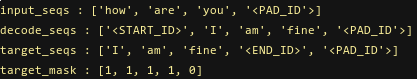
\includegraphics[width=0.222\textwidth]{data_format.png}
	\caption{data format}
\end{figure}


\subsection{\textbf{Database (MongoDB)}}
MongoDB is a document-store database designed for best scalability, high availability and good performance. It allows data persistence in a nested state and has the ability to query the nested data in an undefined fashion with embedded queries. In addition, it does not inflict schema, allowing it to adapt quickly as applications. Moreover, a MongoDB document can contain field types that other documents of the same collection do not have. Anyhow of this flexibility, MongoDB still ensures expected functionalities such as full query language and consistency.\\
MongoDB is in the forefront of NoSQL databases, providing agility and scalability to businesses. More than thousand companies and new start-up companies have acquire and are using MongoDB to develop new applications as it refines client experience, speeds up marketing time and minimize costs. Most bigger web applications like Facebook, Amazon, Google etc. are practitioners of MongoDB. \\

\begin{figure}[!ht]
	\centering
	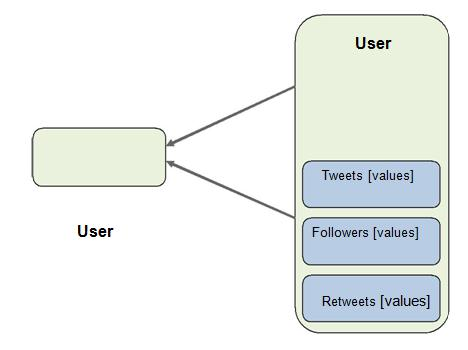
\includegraphics[width=0.45\textwidth]{mongo.png}
	\caption{Demonstration of MongoDB\cite{b7}}
\end{figure}

MongoDB stores data as document in a binary-encoded form called BSON or simply Binary JSON. Like in relational databases, MongoDB organizes documents that tend to have similar structure as collections. A Collection in MongoDB corresponds to a table in relational databases, a document is a row, and a field is a column.\\

Let us consider the data model for a twitter clone application is a example for understanding. A relational database will model the data as multiple tables of User, Followers, Tweets and Retweets. However, in MongoDB Database content, the data could be represented as a single collection of Users. Each User’s document may be contain followers, Tweets, Retweets, represented as an embedded array because in MongoDB Database joins, like inner join and outer joins, doesn't work. In order words, while information of a each different record in relational databases is usually spread across multiple tables with multiple row and column, MongoDB may have all data of a particular record in a single document.

\begin{figure}[!ht]
	\centering
	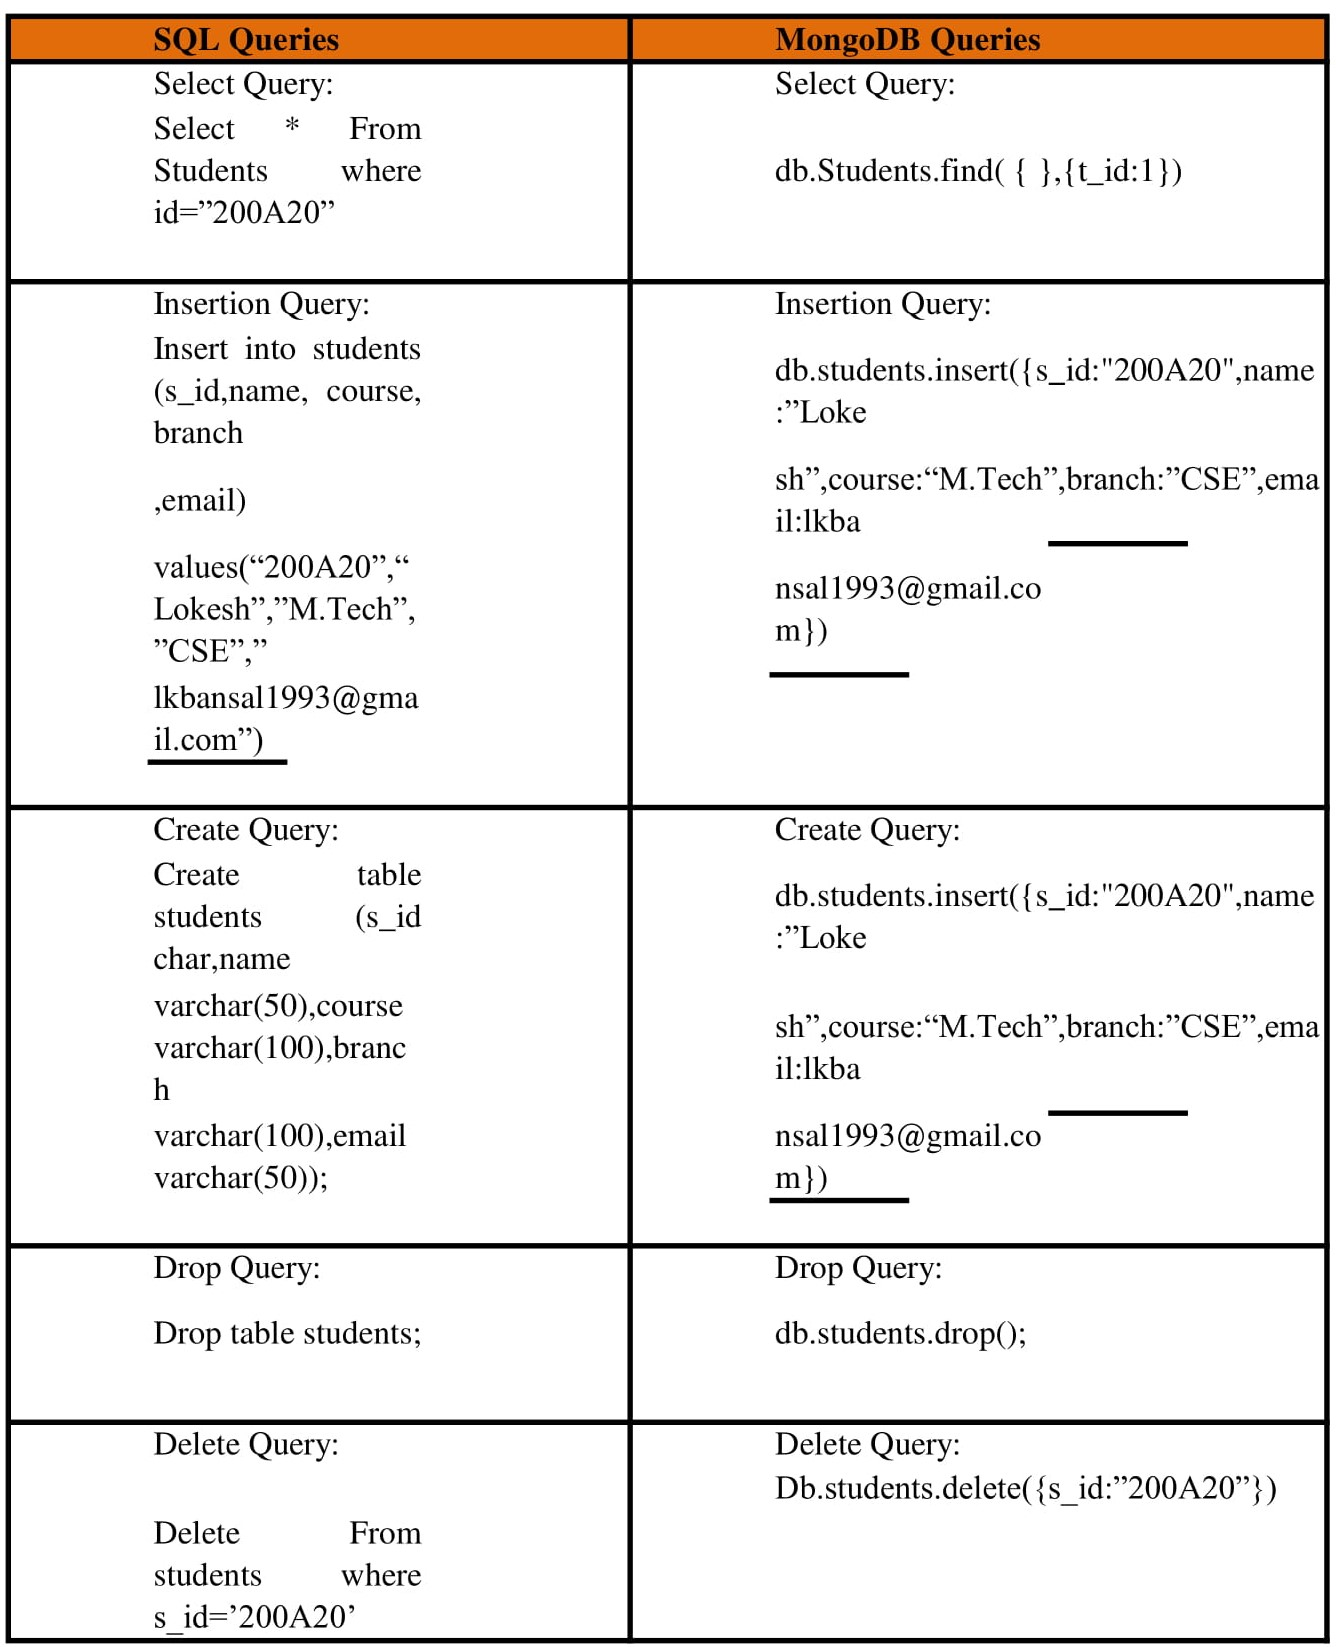
\includegraphics[width=0.45\textwidth]{table-1.jpg}
\end{figure}

The above table shows difference between SQL queries and NoSQL(MongoDB) queries\cite{b7}.\\

\textit{Dynamic Schema:}\\
The structure of a MongoDB document can vary from document to document in the form of JSON, unlike in a relational database where the structure for a row must be defined. For instance, all documents describing Twitter Users might contain user ID, tweets and followers. However, some documents do not necessarily have to require user ID for one or more third-party applications. Hence, fields can be added to a document if needed, without disrupting other documents or updating the central system catalog or having system downtime.
 


\subsection{\textbf{Feedback Analysis}}
Restaurants always want their customers to appreciate their food and ambience. This can be achieved by analyzing the feedbacks given by the customer. From this knowledge, restaurants can improve themselves and serve the customers well.\\
Articulating the emotions and feelings with the succor of words makes human beings inimitable. Technobabbly these feelings are known as sentiments and the process of analyzing these sentiments is called Sentiment Analysis/Opinion Mining. Sentiment Analysis is one of the field of Artificial Intelligence.

\subsubsection{\textit{Survey of Product Reviews using Sentiment Analysis:\cite{b8}}
In this paper, author has proposed a technique called sentiment orientation, which automatically finds the frequently used terms for an aspect of a product from online customer reviews. The methodology which is put forward provides an efficient way of predicting the user’s opinion and thereby suggesting them. Classifying the product review/opinion on the basis of positive and negative is the major task in one of the supervised machine learning approach called lexicon based approach. This work is said to be sentiment orientation.\\
The problems which arose are confection (i.e) multiple ways to arrive at the solution and the second one is to deal with the context based words. To overcome these problems, the sentiment orientation algorithm is proposed by the author. It includes two major approaches:
\begin{itemize}
	\item \textit{Corpus based approach:} It is classified as a linguistic based approach and mainly identifies the emotional similarity of the word. It follows 3A perspective which is: Annotation, Abstraction and Analysis.
	\item \textit{Dictionary based approach:} This approach makes use of datasets like wordnet. By using the resources of words provided by wordnet it is possible to identify the large set of text from the comments that are retrieved. Some of the major advantages of this approach include ease of use, increases time efficiency, removes unwanted, duplicate content and the dataset.
\end{itemize}

\begin{figure}[!ht]
	\centering
	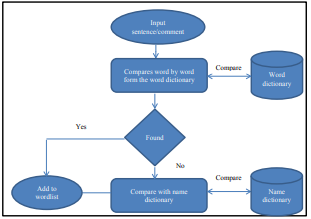
\includegraphics[width=0.5\textwidth]{SO.png}
	\caption{Flowchart for Semantic Orientation}
\end{figure}
Above Figure shows the flowchart explanation for sentiment orientation. Wordlist is the output of this system which is created by comparing words in word dictionary and name dictionary respectively.
\begin{figure}[!ht]
	\centering
	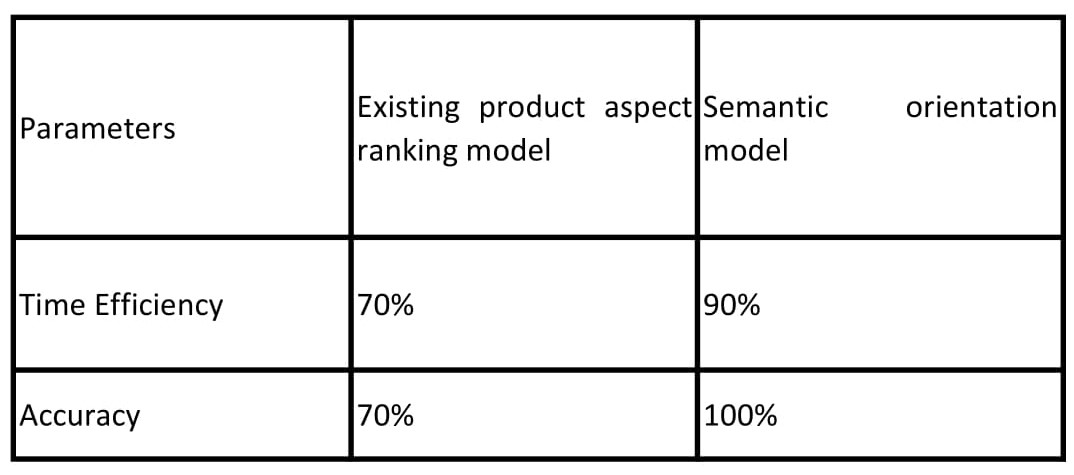
\includegraphics[width=0.5\textwidth]{table2-1.jpg}
\end{figure}

\subsubsection{\textit{Application of Machine Learning Techniques to Sentiment Analysis\cite{b9}}}
Sentiment Analysis/Opinion Mining is the process of identifying whether the user-generated text expresses positive, negative or neutral opinion about an entity which can be product, people, topic, event etc.
In this paper, author has proposed several Sentiment Analysis approaches which include following:
\begin{itemize}
	\item Lexicon Based approach: This approach deals with counting of positive and negative words in the output text. If the text consists of more positive words, then the text is assigned a positive score and if there are more number of negative words, then it is assigned as negative score. There must be some cases where there are equal number of positive and negative words then it is assigned as neutral score. This process is called building an opinion lexicon. Two main approaches for this purpose are:
	\begin{itemize}
		\item Dictionary based approach
		\item Corpus based approach
		
	\end{itemize}
	\item Machine-Learning Based approach: In this approach, dataset is divided into training and testing dataset. Various Machine Learning Algorithms which are usually used for classification of text are: Maximum Entropy, Naïve Bayes, Support vector machines
	\item Hybrid approach: This approach combines both lexicon and machine learning based sentiment analysis techniques. The advantage of this is best of both worlds can be attained.
\end{itemize}
In this paper\cite{b9} author has briefly described each step which needs to be followed for Sentiment analysis procedure, below described steps are applied on twitter dataset, hence describing them in detail- 
\begin{itemize}
	\item Data Collection: Twitter data is collected using Twitter API
	\item Data Preprocessing: Once data is collected using Twitter API, there is so much of noise present in it which needs to be removed for getting good performance. This process of removal of noise from data is called data preprocessing.
	Steps that are carried out in preprocessing are as follows-
	\begin{itemize}
		\item Case Conversion 
		\item Stop-words Removal
		\item Punctuation Removal
		\item Stemming
		\item Lemmatization
		\item Spelling Correction
	\end{itemize}
	\item Feature Extraction: Once tweets are preprocessed, features are extracted which are relevant for sentiment analysis. Some example features are- team presence and frequency, parts of speech tagging, opinion words and phrases, negation, presence of emoticons in tweets, hashtags which are all twitter specific features.
	\item Training and Testing Machine Learning classifier: After features are selected, a Machine Learning classifier is chosen for sentiment Analysis. List of Machine Learning Classifiers:
	\begin{itemize}
		\item Naïve Bayes Classifier
		\item Support vector machines
		\item Decision trees
	\end{itemize}
	
\end{itemize}	
In the paper\cite{b9}, authors have used Apache Spark to obtain quicker results. In the proposed work, analysis is performed on datasets of different sizes and domains to demonstrate that the proposed framework works on data of all sizes and domains. Three different datasets of varying sizes and domains are considered for analysis.\\
The following points can be elaborated based on outcome persual:-
\begin{itemize}
	\item Multinomial Naïve Bayes does not perform as expected when supplied with small training dataset.
	\item Decision tree takes longer training time than Naïve Bayes.
	\item Decision tree takes very less time for predicting unseen data compared to multinomial Naïve Bayes.
	\item Decision tree performs better than Multinomial Naïve Bayes for datasets of varied sizes and domains.
	\item This work uses Apache Spark Cluster for processing. Hence, the proposed framework is able to produce the results of analysis quickly.
\end{itemize}

\subsubsection{\textit{Performance Analysis of Supervised Machine Learning Techniques for Sentiment Analysis\cite{b10}}}
Human beings always tries to make the machine smarter to solve all its problem smartly and efficiently with in some stipulated period of time. Therefore, machine learning techniques come to action by using which machines get trained and expected to work accordingly. Machine Learning (ML) is a field of Computer Science in which machines of computers are able to learn without being programmed explicitly. \\
\begin{figure}[!ht]
	\centering
	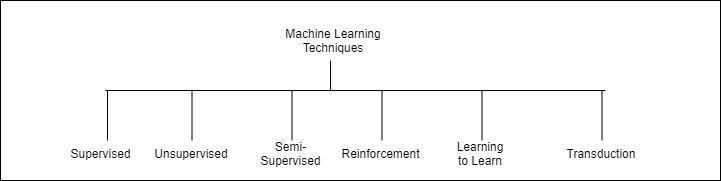
\includegraphics[width=0.5\textwidth]{tech.png}
\end{figure}
In \cite{b10} author has proposed a methodology where Sentiment Analysis is done on movie reviews. Step-by-Step procedure for the same is described below:
\begin{itemize}
	\item Collecting Movie Reviews Data Sets
	\item Cleaning the Data Sets: Characters, numbers, special characters, and unrecognized characters are all removed from the dataset, this process is called cleaning or pre-processing of data.
	\item Data Categorization: Supervised Machine Learning technique take labelled data, which needs categorizing the data into positive or negative. In this, author has used python for labelling the data.
	\item Preparing training and testing datasets: 70\% of data is considered as training dataset and 30% as testing data
	\item Training the Model with training Data Sets
	\begin{figure}[!ht]
		\centering
		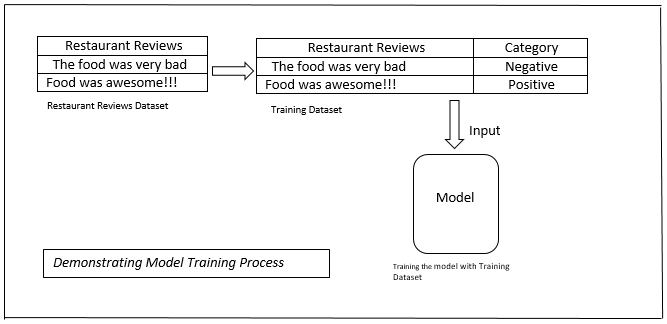
\includegraphics[width=0.5\textwidth]{train.png}
	\end{figure}
	\item Testing the Model with Training DataSets 
	\begin{figure}[!ht]
		\centering
		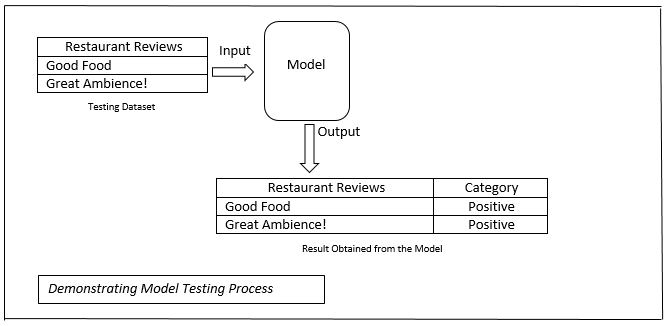
\includegraphics[width=0.5\textwidth]{test.png}
	\end{figure}
\end{itemize}
Result:
	\begin{figure}[!ht]
	\centering
	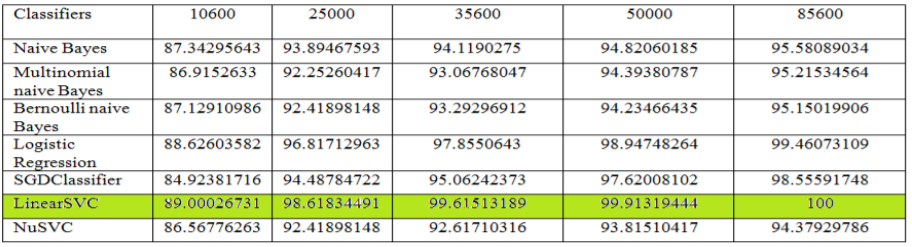
\includegraphics[width=0.5\textwidth]{result.png}
\end{figure}
The above table shows the experimental results of 6 classifiers. From which LinearSVC performs the best.

\subsection{\textbf{Speech Synthesis}}
Speech synthesis is the artificial production of human speech. A computer system used for this purpose is called a speech computer or speech synthesizer, and can be implemented in software or hardware products. A text-to-speech (TTS) system converts normal language text into speech.A text to speech output is based on generating corresponding sound output when the text is inputted \cite{b11}.Wide range of applications use text to speech technique in medicals, telecommunications fields, etc. Each spoken word is created from the phonetic combinationof a set of vowel and consonant speech sound units. Producing an artificial human speech is known as speech synthesis.  
\begin{figure}[!ht]
	\centering
	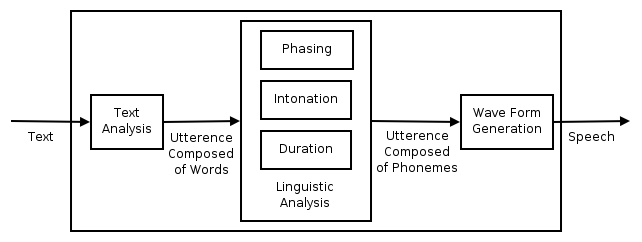
\includegraphics[width=0.5\textwidth]{SpSy.png}
	\caption{Speech Synthesis Module\cite{b12}}
\end{figure}
The Various speech synthesis methods that have been used for text to speech output for obtaining intelligible and natural output are Concatenative, Formant, Articulatory, Hidden Markov model (HMM). 


\section{Proposed Work}
The system first analyzes the speech given by the user. The google text to speech algorithm in python (https://pypi.org/project/gTTS/) will convert the spoken sentence into a text format . Once the speech format is converted into text, the text will be sent to the rule based system for proccessing, this request will be sent using a post request (rest api) which will take an input of the text as the headers and return multiple attributes such as the response, intent as well as entities .Our system will then process the text and detect intents out of the given input, generating an apt response for the user query.Meanwhile based on the given intent the order and the bill will be recorded for futher storage into the database.Once the user is done with his food he will be given an option to give a feedback about his experience, during this time the user will also be prompted about his total bill. The bill will be calcualted by getting the default prices from the mongodb server and multplying them by thier quantities. If the user feels like giving a feedback, the feedback will be processed. 
\begin{figure}[h!]
	\centering
	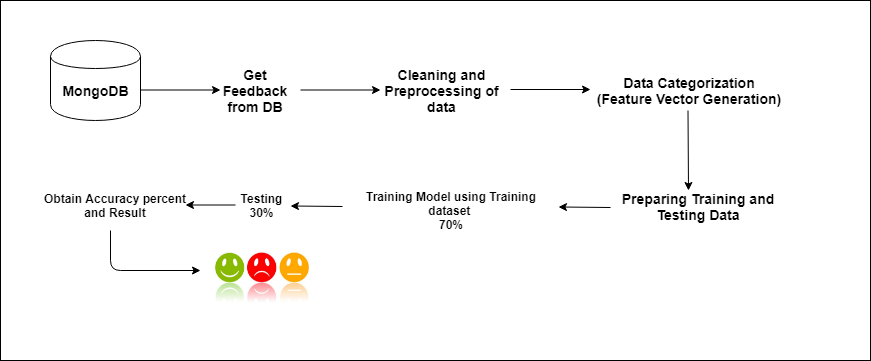
\includegraphics[width=0.5\textwidth]{SA.png}
	\caption{Steps for Feedback Analysis}
\end{figure}
Feedback Analysis/ Sentiment Analysis is done using nltk with python 3.5.2, using spyder ide, preprocessing steps performed are[14]:\\
	1. Tokenizing\\
	2. Stop Words\\
	3. Stemming\\
	4. Part of Speech Tagging\\
	5. Chunking\\
	6. Lemmatizing\\
	7. Named Entity Recognition\\
The Dataset which is used for training and testing, is taken from nltk corpora. Words are converted to featuresets, to compare with the test data. Classifiers which are used for classifying the text are:
    \textit{1. Naive Bayes(original):} \\
	It is a classification technique based on Bayes’ Theorem with an assumption of independence among predictors. In simple terms, a Naive Bayes classifier assumes that the presence of a particular feature in a class is unrelated to the presence of any other feature.\\\\
    \textit{2. Multinominal Naive Bayes:}\\ 
	It is used for discrete counts. For example, let’s say,  we have a text classification problem. Here we can consider bernoulli trials which is one step further and instead of “word occurring in the document”, we have “count how often word occurs in the document”, you can think of it as “number of times outcome number x\_i is observed over the n trials”.\\\\
    \textit{3. Bernoulli Naive Bayes: }\\
	The binomial model is useful if your feature vectors are binary (i.e. zeros and ones). One application would be text classification with ‘bag of words’ model where the 1s \& 0s are “word occurs in the document” and “word does not occur in the document” respectively.\\\\
	\textit{4. Linear Regression:} \\
	In this technique, the dependent variable is continuous, independent variable(s) can be continuous or discrete, and nature of regression line is linear.Linear Regression establishes a relationship between dependent variable (Y) and one or more independent variables (X) using a best fit straight line (also known as regression line).\\
	It is represented by an equation Y=a+b*X + e, where a is intercept, b is slope of the line and e is error term. This equation can be used to predict the value of target variable based on given predictor variable(s).\\\\
	\textit{5. SGD() Classifier: }\\
	Stochastic Gradient Descent (SGD) is a simple yet very efficient approach to discriminative learning of linear classifiers under convex loss functions such as (linear) Support Vector Machines and Logistic Regression.\\\\
	\textit{6. SVC:} \\
	Uses one-against-one approach\\\\
	\textit{7. Linear SVC: }\\
	Uses one-against-rest approach\\\\
	\textit{8. NuSVC:} \\
	The nu-SVM has the advantage of using a parameter nu for controlling the number of support vectors. The parameter nu represents the lower and upper bound on the number of examples that are support vectors and that lie on the wrong side of the hyperplane, respectively. 
\\\\\\
Python library called 'Pickle' is used for storing the classifiers so that we dont need to run the classifiers again and again. 'Voted Classifier' is used as a highlight of the system, where the highest vote is taken from the above defined classifiers and given as the output.

\bigskip

The generated query will then be converted into speech again using the Espeak module. Once the user is done with everything his details are stored in the database with attribuites such as:\\
* total bill\\
* name\\
* feedback\\
* sentiment processed\\

\section{Results and Discussion}
\begin{figure}[!ht]
	\centering
	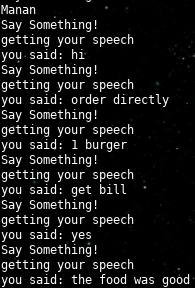
\includegraphics[width=0.2\textwidth]{input.png}
	\caption{Chat between Customer and Device}
\end{figure}
\begin{figure}[!ht]
	\centering
	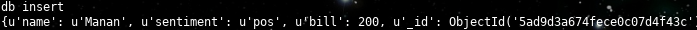
\includegraphics[width=0.5\textwidth]{output.png}
	\caption{Sentiment Analysis of Feedback}
\end{figure}
\begin{figure}[!ht]
	\centering
	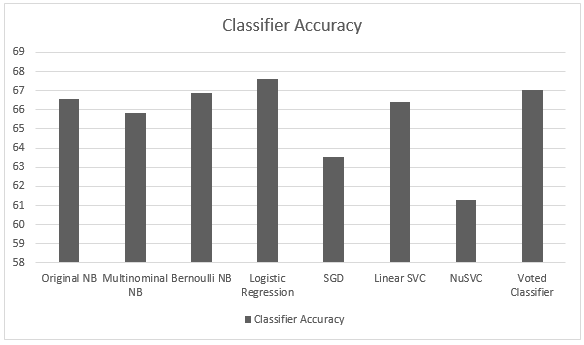
\includegraphics[width=0.5\textwidth]{R2.png}
	\caption{Graphical representation of all classifiers performance comparison}
\end{figure}

From the above result, we can see that out of all the classifiers compared, Multinominal Naïve Bayes gives highest accuracy. It is explicitly dependent on the size of the dataset used for training and testing. 

\section{Conclusion}
 People feel more laid-back when they are interacting with the system in a familiar human-like language.Furthermore, with the proliferation of Smart Speakers like Amazon Echo, Google Home, Apple Homepod, the use of voice is starting to become a new trend. And hence our project tries to solve the above issues in a restaurant management space where there is a need for automation as humans may be bottlenecking the limits of the system. Based on the thorough study of various different technologies during the semester we can say that an Object-oriented database (MongoDB) is way more efficient than a normal SQL database. We have also compared different ML Classifiers used to carry out Text Classification in sentiment analysis on our feedback system. In the end, we can successfully conclude that Restaurant management system using modern technologies like NLP, RBS, ML, etc is way more effective and systematic than traditional restaurant management systems. 

\section{Future Work}

	In future, by following the footprints of different data analysis algorithms, we plan to propose a system which would be the combination of restaurant management  system and inventory management of the restaurant. 
	Furthermore, restaurant can get the information about the price ranges, popular food items, recommendations for the customers during their next visit, and also improvements to be considered, through feedback analysis.
	

\begin{thebibliography}{00}
 \bibitem{b1}ASR [Online] Available:http://support.docsoft.com/help/whitepaper-asr.pdf (2018, April 21)  
  \bibitem{b2} MFCC [Online] Available:https://en.wikipedia.org/wiki/Mel-frequency-cepstrum (2018, April 21) 
  \bibitem{b3} Speech Recognition [Online] (2018, April 21) Available:http://what-when-how.com/video-search-engines/speech-recognition-audio-processing-video-search-engines/
  \bibitem{b4} Available:https://medium.com/@abraham.kang/understanding-the-differences-between-alexa-api-ai-wit-ai-and-luis-cortana-2404ece0977c(2018, April 21)
  \bibitem{b5} https://cs224d.stanford.edu/lectures/CS224d-Lecture2.pdf(2018, April 21)
  \bibitem{b6} http://building-babylon.net/2015/07/29/glove-global-vectors-for-word-representations/(2018, April 21)
  \bibitem{b7} Lokesh Kumar, Dr. Shalini Rajawat,Krati Joshi, "Comparative analysis of NoSQL (MongoDB) with MySQL Database", International Journal of Modern Trends in Engineering and Research
  \bibitem{b8} R. Jenitha Sri, P. Ajitha, "Survey of Product Reviews using Sentiment Analysis", International Journal of Science and Technology
 \bibitem{b9} Anuja P.Jain, Asst. Prof Padma Dandannavar, "Application of Machine Learning Techniques to Sentiment Analysis", IEEE 2016
 \bibitem{b10}BiswaRanjanSamal, Anil Kumar Behera, Mrutyunjaya Panda, “Performance Analysis of Supervised Machine Learning Techniques for Sentiment Analysis”, IEEE 3rd International Conference on Sensing, Signal Processing and Security(ICSSS)
 \bibitem{b11}  Sneha Lukose, Savitha S. Upadhya,"Text to Speech Synthesizer-Formant Synthesis", International Conference on Nascent Technologies in the Engineering Field, IEEE 2017 (2018, April 21) 
 \bibitem{b12}Text to Speech Flow [Online] Available: http://www.wezs.com/~danguy/monguy/TTS.html (2018, April 21) 
 \bibitem{b13}Speech Synthesis [Online] Available: https://en.wikipedia.org/wiki/Speech.synthesis (2018, April 21) 
 \bibitem{b14}Eril Cambria, Soujanya Poria, Alexander Gelbukh, Mike Thelwall, “Sentiment Analysis Is a Big Suitcase”, IEEE 2017
 
 \end{thebibliography}
\end{document}